\documentclass[pdftex, a4paper,12pt, oneside, svgnames]{article}

\usepackage[usenames,dvipsnames,svgnames,table]{xcolor}
\usepackage[left=3cm,text={15.25cm,23cm},top=3cm]{geometry}
\usepackage[T1]{fontenc}
\usepackage[utf8]{inputenc}

\usepackage{pslatex} % to use PostScript fonts
\usepackage[pdftex]{graphicx}

\usepackage{listings}
\usepackage{enumerate}
\usepackage{epsfig}
\usepackage{amsfonts}
\usepackage{amsmath}
\usepackage{fancyhdr}
\usepackage[center]{caption}

\catcode`\_=12 % no need to escape (\_) underscores, isn't it dangerous?

\usepackage{url}
\usepackage{hyperref}
\hypersetup{
	colorlinks,
	linkcolor={black},
	citecolor={green},
	urlcolor={blue}
}

\usepackage{amssymb} % http://ctan.org/pkg/amssymb
\usepackage{pifont} % http://ctan.org/pkg/pifont
\newcommand{\cmark}{\ding{51}}%
\newcommand{\xmark}{\ding{55}}%

\makeatletter
\newcommand\HUGE{\@setfontsize\Huge{50}{60}}
\makeatother

\renewcommand*\familydefault{cmss}

\begin{document}

%-----------------------------------------------------------------------------
%  Title page
%-----------------------------------------------------------------------------

\begin{titlepage}
\begin{center}

\fontfamily{cmss}


\includegraphics[width=12cm]{figures/avast-logo-cmyk}

\vfill

{\LARGE Retargetable Decompiler's IDA Plugin}
\\[5 mm]
{\HUGE User Guide}
\\[3 mm]
{\large Version 0.4}

\vfill

{\LARGE
\href{https://github.com/avast-tl/retdec-idaplugin}{https://github.com/avast-tl/retdec-idaplugin} \\[2 mm]
\href{https://retdec.com}{https://retdec.com} \\[2 mm]
\href{mailto:support@retdec.com}{support@retdec.com} \\[4 mm]
\today}

\end{center}
\end{titlepage}

%-----------------------------------------------------------------------------
%  Content
%-----------------------------------------------------------------------------

\tableofcontents
%\listoffigures
%\listoftables

%-----------------------------------------------------------------------------
%  Introduction
%-----------------------------------------------------------------------------
\newpage
\section{Introduction}
\label{sec:introduction}
This document describes the Retargetable Decompiler's plugin for IDA (RetDec plugin). Its goal is to integrate with IDA, give transparent access to the Retargetable Decompiler and provide user-interaction capabilities like navigation or code refactoring. An example of code decompiled by Retdec plugin is shown in Figure~\ref{fig:overview}.

Retargetable Decompiler (RetDec) is a reverse-engineering tool independent of any particular target architecture, file format, operating system, or compiler. It was developed in cooperation of Faculty of Information Technology, Brno University of Technology and AVG Technologies. Since the acquisition of AVG Technologies by Avast in 2016, Avast has continued to develop the decompiler. It is using Capstone disassembler engine and a Capstone2LlvmIR library to translate machine code into a high-level-language representation. Currently, the decompiler supports the MIPS, ARM (including Thumb extension), x86, and PowerPC architectures using the Windows PE, COFF, Unix ELF, Intel HEX, and RAW binary file formats.

RetDec can be used in the following ways:
\begin{enumerate}
	\item Online decompilation using \href{https://retdec.com/decompilation/}{web interface}.
	\item Remote decompilation using \href{https://retdec.com/api/}{Application programming interface} (API).
	\item Local build:
	\begin{enumerate}
		\item Compiling \href{https://github.com/avast-tl/retdec}{RetDec repository} on your own.
		\item Downloading and installing \href{https://github.com/avast-tl/retdec/releases}{RetDec binary release}.
	\end{enumerate}
	\item \href{https://retdec.com/idaplugin/}{RetDec IDA plugin} (this quide's topic):
	\begin{enumerate}
		\item Remote decompilation using API.
		\item Local decompilation using local build.
	\end{enumerate}
\end{enumerate}

\begin{figure}[!ht]
	\centering
	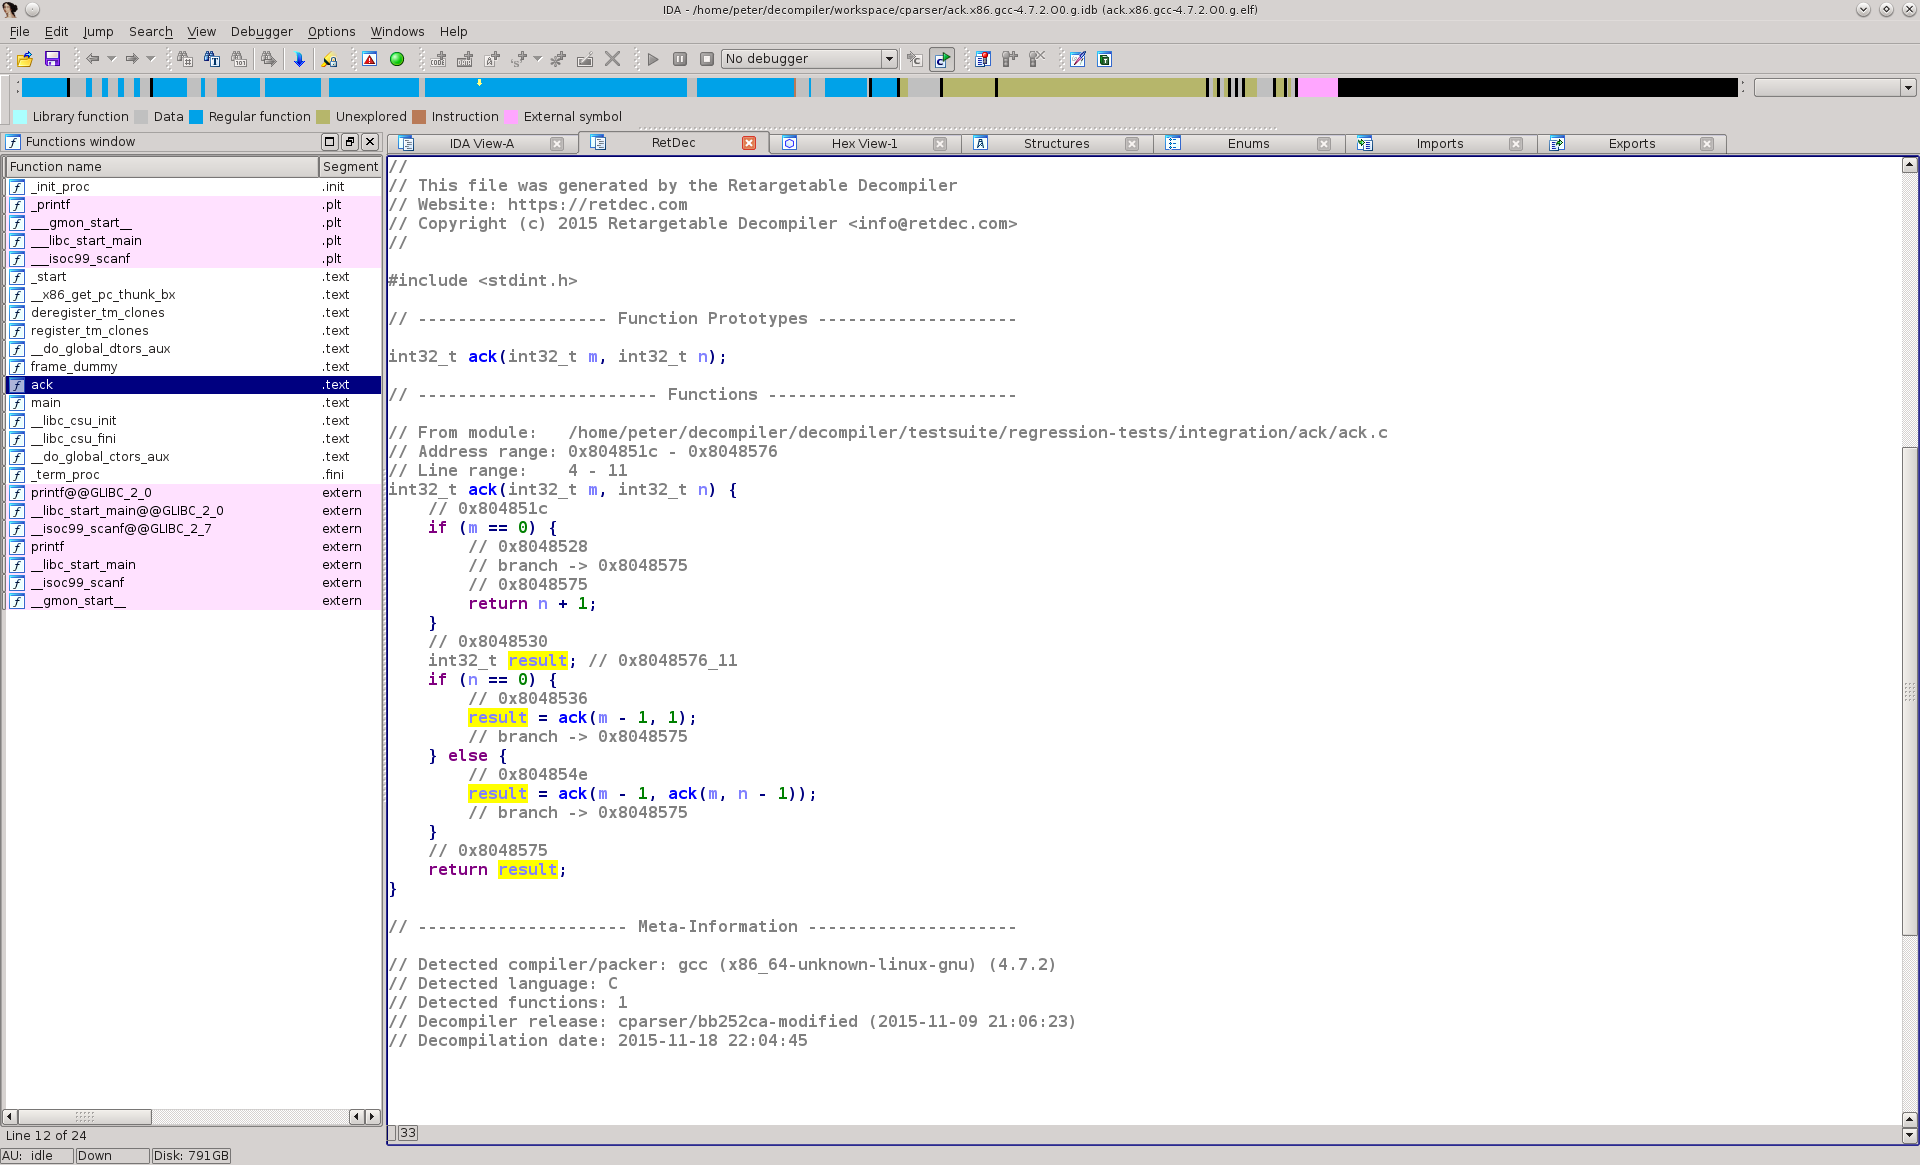
\includegraphics[width=\textwidth]{figures/overview}
	\caption{Example of code decompiled by RetDec plugin.}
	\label{fig:overview}
\end{figure}

%-----------------------------------------------------------------------------
%  Installation
%-----------------------------------------------------------------------------
\newpage
\section{Installation}
\label{sec:installation}
This section describes prerequisites and the installation process of RetDec IDA plugin binary release.

It is also possible to build and install the plugin directly from sources. To do so, follow the \href{https://github.com/avast-tl/retdec-idaplugin#build-and-installation}{Build and Installation} instructions instead of this section.

\subsection{IDA}
The plugin is created using IDA SDK version 6.6. The plugin is compatible with the following IDA versions: 6.6, 6.7, 6.8, 6.9, 6.95. The plugin does NOT work with IDA 7.x.

\subsection{Linux}
Follow the next steps to install RetDec plugin in a Linux environment:
\begin{enumerate}
	\item Install 32-bit versions of the following shared-object dependencies:
\begin{verbatim}
libc.so.6 libgcc_s.so.1 libm.so.6 libpthread.so.0 libstdc++.so.6
\end{verbatim}
	\item Download the Linux installation package (Table~\ref{table:installation-package-linux}) from the \href{https://github.com/avast-tl/retdec-idaplugin/releases}{project's release page}.
	\item Copy \texttt{retdec.plx} to the IDA's plugin directory (\texttt{<IDA\_ROOT>/plugins}).
\end{enumerate}

\begin{table}[!ht]
\centering
\caption{Linux installation package contents.}
\label{table:installation-package-linux}
\begin{tabular}{ll}
\textbf{File} & \textbf{Description}\\
\hline
\texttt{license} & Directory with licenses. \\
\texttt{license/LICENSE} & RetDec IDA plugin's license. \\
\texttt{license/LICENSE-THIRD-PARTY} & Licenses of libraries used by RetDec plugin. \\
\texttt{retdec.plx} & 32-bit Linux RetDec plugin. \\
\texttt{user_guide.pdf} & RetDec plugin's user guide (this document). \\
\end{tabular}
\end{table}

\subsection{Windows}
\label{sec:installation:windows}
The Windows version of the plugin requires Windows 7 or later, with the MSVC 2015 runtime\footnote{Visual C++ Redistributable for Visual Studio 2015: \url{https://www.microsoft.com/en-us/download/details.aspx?id=48145}} installed.

Follow the next steps to install RetDec plugin in a Windows environment:
\begin{enumerate}
	\item Download the Windows installation package (Table~\ref{table:installation-package-windows}) from the \href{https://github.com/avast-tl/retdec-idaplugin/releases}{project's release page}.
	\item Copy \texttt{retdec.plw} to the IDA's plugin directory (\texttt{<IDA\_ROOT>/plugins}).
\end{enumerate}

\begin{table}[!ht]
\centering
\caption{Windows installation package contents.}
\label{table:installation-package-windows}
\begin{tabular}{ll}
\textbf{File} & \textbf{Description}\\
\hline
\texttt{license} & Directory with licenses. \\
\texttt{license/LICENSE} & RetDec IDA plugin's license. \\
\texttt{license/LICENSE-THIRD-PARTY} & Licenses of libraries used by RetDec plugin. \\
\texttt{retdec.plw} & 32-bit Windows RetDec plugin. \\
\texttt{user_guide.pdf} & RetDec plugin's user guide (this document). \\
\end{tabular}
\end{table}

\subsection{Windows Plugin on Linux}
It is also possible to run the Windows version of IDA with the Windows version of RetDec plugin on Linux using Wine\footnote{\url{https://www.winehq.org/}}. Install RetDec plugin as described in Section~\ref{sec:installation:windows} and if it does not run out of the box, try a workaround\footnote{\url{https://bugs.winehq.org/show_bug.cgi?id=39437\#c6}}.

%-----------------------------------------------------------------------------
%  Configuration
%-----------------------------------------------------------------------------
\section{Configuration}
\label{sec:configuration}
This section describes how to configure RetDec plugin. After you follow these steps, you should have your plugin ready for work.

\subsection{IDA's plugin.cfg}
\label{sec:config:plugin-cfg}
The plugin's default mode is set to selective decompilation (see Section~\ref{sec:decompilation}). It tries to register hotkey \texttt{CTRL+D} for its invocation. If you already use this hotkey for another action or you just want to use a different hotkey, you need to modify IDA's plugin configuration file. Moreover, the plugin supports one more decompilation mode and a hotkey invocation for the plugin's configuration. If you want to use any of them, you also have to modify the config file.

The IDA's plugin configuration file is in \texttt{<IDA\_ROOT>/plugins/plugins.cfg}. Its format is documented inside the file itself. To configure RetDec plugin, add the following lines at the beginning\footnote{Newer versions of IDA behave strangely when the lines are appended at the end, so just put them at the start.} of the file:
\begin{verbatim}
; Plugin_name           File_name Hotkey        Arg
; -------------------------------------------------
Retargetable_Decompiler retdec    Ctrl-d        0
Retargetable_Decompiler retdec    Ctrl-Shift-d  1
Retargetable_Decompiler retdec    Ctrl-Shift-c  2
\end{verbatim}
These lines tell IDA which hotkeys invoke the plugin and what argument is passed to it. The plugin's behavior after invocation is determined by the passed argument. Possible argument values are summarized in Table~\ref{table:plugin-args}. In the provided example, we mapped selective decompilation to hotkey \texttt{CTRL+D} (plugin's default), full decompilation to \texttt{CTRL+SHIFT+D}, and plugin configuration to \texttt{CTRL+SHIFT+C}. However, you may choose whichever hotkeys you like, provided they do not clash with other plugins or IDA.

\begin{table}[!ht]
\centering
\caption{Description of RetDec plugin's invocation arguments.}
\label{table:plugin-args}
\begin{tabular}{cl}
\textbf{Argument value} & \textbf{Description}\\
\hline
\texttt{0} & Invokes selective decompilation. See Section~\ref{sec:decompilation}. \\
\texttt{1} & Invokes full decompilation. See Section~\ref{sec:decompilation}. \\
\texttt{2} & Invokes plugin configuration inside IDA. See Section~\ref{sec:config:from-ida}.
\end{tabular}
\end{table}

\subsection{Decompilation Configuration}
Each time a decompilation is triggered, plugin checks that it is properly configured. If it is not, warning shown in Figure~\ref{fig:config-warning} is displayed. After you hit \texttt{OK}, the configuration dialog (Figure~\ref{fig:config-dialog-1}) appears. Here, you can choose the decompilation mode to use:
\begin{enumerate}
	\item Remote API decompilation (plugin's default) -- you have to provide your API key. To access it, register to \url{https://retdec.com}, login, and click on \texttt{Account}.
	\item Local decompilation -- you have to install \href{https://github.com/avast-tl/retdec}{RetDec} local build and make sure plugin finds the \texttt{decompile.sh} script. Either add the decompiler's \texttt{bin} directory to the system \texttt{PATH}, or set path to \texttt{decompile.sh} in the form as shown in Figure~\ref{fig:config-dialog-2}.
\end{enumerate}

The settings will be saved and if you want to change them later, you need to manually invoke the plugin's configuration from IDA (see Section~\ref{sec:config:from-ida}).

\begin{figure}[!ht]
	\centering
	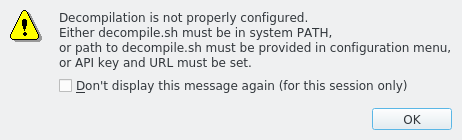
\includegraphics[width=10cm]{figures/config-warning}
	\caption{RetDec plugin's configuration warning.}
	\label{fig:config-warning}
\end{figure}

\begin{figure}[!ht]
	\centering
	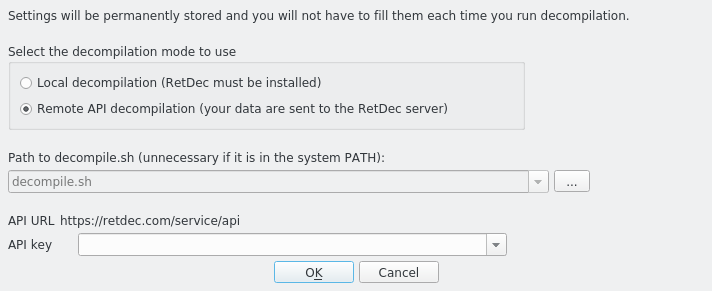
\includegraphics[width=13cm]{figures/config-1}
	\caption{RetDec plugin's configuration dialog.}
	\label{fig:config-dialog-1}
\end{figure}

\begin{figure}[!ht]
	\centering
	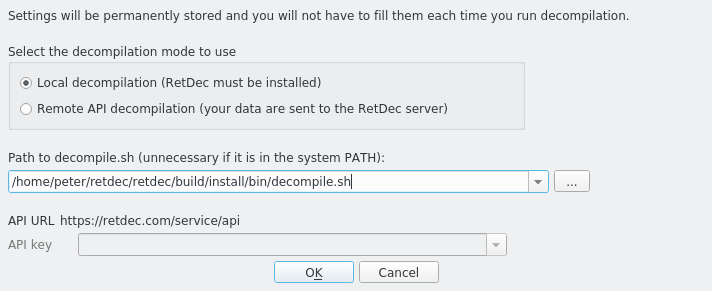
\includegraphics[width=13cm]{figures/config-2}
	\caption{RetDec plugin's configuration dialog -- path to \texttt{decompile.sh} set.}
	\label{fig:config-dialog-2}
\end{figure}

\subsection{Configuration from IDA}
\label{sec:config:from-ida}
The same dialog (Figure~\ref{fig:config-dialog-1}) that is displayed if the plugin is misconfigured can be opened from IDA anytime later. There are the following two ways to do it:
\begin{itemize}
	\item If you configured a hotkey for the plugin's configuration argument value according to Section~\ref{sec:config:plugin-cfg}, you can use it to invoke the configuration dialog.
	\item You can also open the configuration dialog from the \texttt{Options/RetDec plugin options} menu (Figure~\ref{fig:config-menu}).
\end{itemize}

\begin{figure}[!ht]
	\centering
	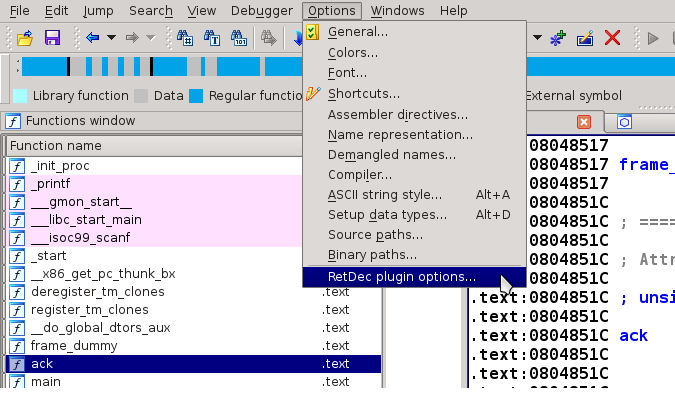
\includegraphics[width=12cm]{figures/menu-config-cut}
	\caption{Opening the plugin's configuration dialog from the menu.}
	\label{fig:config-menu}
\end{figure}

%-----------------------------------------------------------------------------
%  Plugin Information
%-----------------------------------------------------------------------------
\section{Plugin Information}
\label{sec:plugin-info}
This section describes how to find information about RetDec plugin you are currently using and how the plugin communicates information to you.

\subsection{About Plugin}
Information about RetDec plugin can be found among IDA's information on the registered plugins at \texttt{Help/About program} (Figure~\ref{fig:about-ida}), where you need to click on the \texttt{Addons} button (Figure~\ref{fig:addons}). Then, find the \texttt{Retargetable Decompiler} entry in the presented list (Figure~\ref{fig:plugin-info}).

\begin{figure}[!ht]
	\centering
	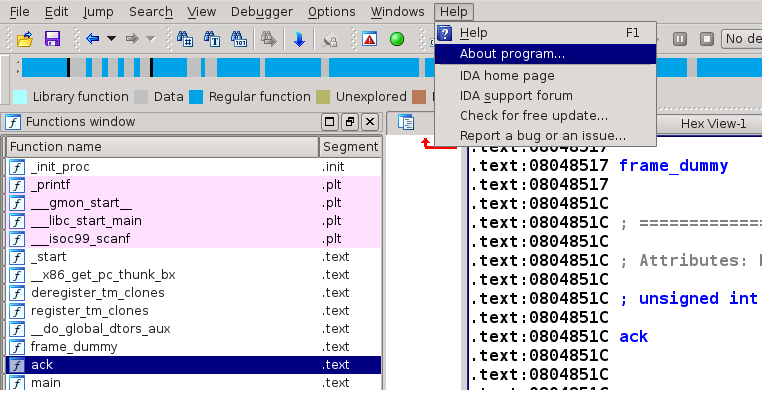
\includegraphics[width=12cm]{figures/help-about-program-cut}
	\caption{Opening the About IDA dialog from the menu.}
	\label{fig:about-ida}
\end{figure}

\begin{figure}[!ht]
	\centering
	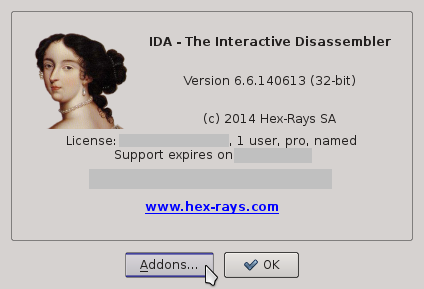
\includegraphics[width=10cm]{figures/addons}
	\caption{Information window about IDA.}
	\label{fig:addons}
\end{figure}

\begin{figure}[!ht]
	\centering
	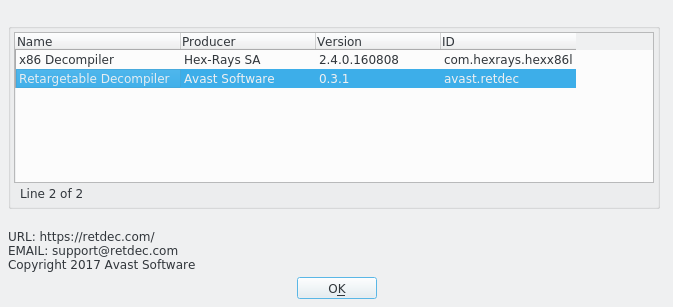
\includegraphics[width=10cm]{figures/plugin-info}
	\caption{Information window about RetDec plugin.}
	\label{fig:plugin-info}
\end{figure}

\subsection{Output Window}
Right after the start, as well as during the work with RetDec plugin, it communicates with you mainly through the IDA's output window (Figure~\ref{fig:ida-output-window}). Here, you are shown several kinds of important messages:
\begin{verbatim}
[RetDec info]   :    some important piece of information
[RetDec warning]:    something went a little bit wrong
[RetDec error]  :    something went very wrong
\end{verbatim}

\begin{figure}[!ht]
	\centering
	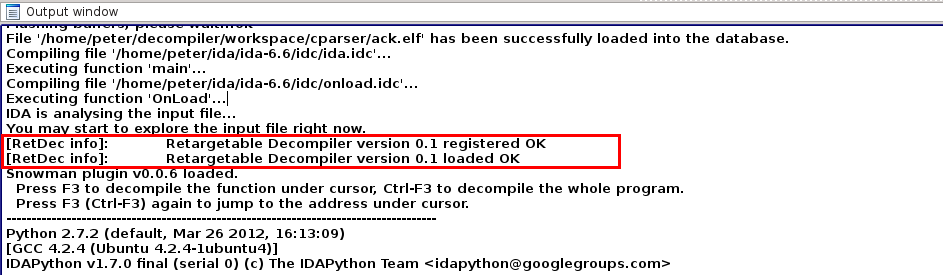
\includegraphics[width=13cm]{figures/ida-output-window-highlighted}
	\caption{IDA's output window.}
	\label{fig:ida-output-window}
\end{figure}

\subsection{GUI Windows}
Sometimes, RetDec plugin wants to be sure you noticed an important message or event. In such a case, it shows you a pop-up window, which forces you to acknowledge it by pressing \texttt{OK} or a similar button.

%-----------------------------------------------------------------------------
%  Decompilation
%-----------------------------------------------------------------------------
\section{Decompilation}
\label{sec:decompilation}
This section describes how to invoke a decompilation. After reading it, you should be able to decompile a selected function, as well as an entire binary that is being analyzed.

\subsection{Selective Decompilation}
\label{sec:selective-decompilation}
RetDec plugin's primary decompilation mode is selective decompilation. It decompiles the function that is currently under the cursor. It is invoked from the IDA's disassembly window, where you need to bring focus to the desired function and use either the default hotkey \texttt{CTRL+D}, or a hotkey you configured according to Section~\ref{sec:config:plugin-cfg}.

Once the decompilation is finished, the decompiled source code is displayed in a new IDA viewer window. Here, you can invoke new decompilations by double-clicking on function calls.

\subsection{Full Decompilation}
If you configured a hotkey for full decompilation in Section~\ref{sec:config:plugin-cfg}, you can use it to decompile an entire binary that is being analyzed. The result of this decompilation is stored into an output file, whose location is communicated to you through IDA's output window. The result cannot be displayed in the IDA's viewer window.

%-----------------------------------------------------------------------------
%  User Interactions
%-----------------------------------------------------------------------------
\section{User Interactions}
\label{sec:user-interactions}
This section describes various kinds of user interactions that are currently supported by RetDec plugin. As was stated in Section~\ref{sec:decompilation}, these interactions are applicable only on results from selective decompilations because full decompilations cannot be displayed in IDA's viewer window.

\subsection{Basic Interactions}
We use the IDA's native custom viewer window to display the decompiled source codes. Therefore, the plugin feels like part of IDA and we get a word occurrences highlighting (Figure~\ref{fig:occurrence-highlighting}) out of the box.

\begin{figure}[!ht]
	\centering
	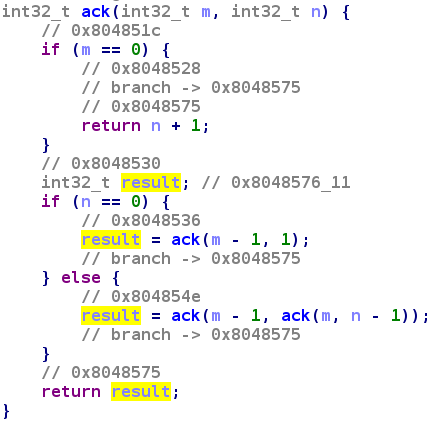
\includegraphics[width=8cm]{figures/occurrence-highlighting}
	\caption{Native word occurrence highlighting.}
	\label{fig:occurrence-highlighting}
\end{figure}

\subsection{Navigation}
\label{sec:navigation}
RetDec plugin supports function navigation---jumping forward and backward between already decompiled functions, or invoke an entirely new decompilation. When you double-click on a function call, the plugin presents the requested function. If it was already decompiled in the past, the cached result is shown to perform the action faster. You have to either explicitly request a re-decompilation of the previously processed functions, or perform an action that triggers the re-decompilation automatically (see Section~\ref{sec:refactoring}). Re-decompilation can be forced by using the selective decompilation hotkey in IDA's disassembly (re-decompilation of any function), or in the RetDec plugin's viewer window (re-decompilation of currently shown function). If the double-clicked function was not decompiled yet, it is selectively reversed and displayed. In either case, only one function is shown at a time. A navigation entry for the newly presented function is added into a doubly linked navigation list, right after the entry for function from which the invocation was made. The list is then used for forward and backward navigation between the stored functions. An example of such navigation is depicted in Figure~\ref{fig:navigation}.

\begin{figure}[!ht]
	\centering
	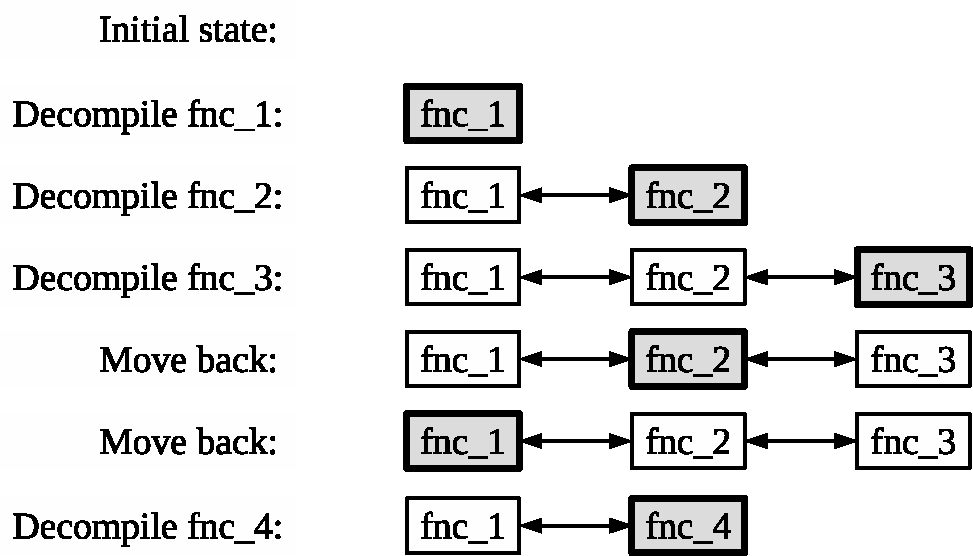
\includegraphics[width=8cm]{figures/navigation}
	\caption{Decompiled function navigation example.}
	\label{fig:navigation}
\end{figure}

Unfortunately, we were not able to integrate navigation with IDA's graphical control elements, so it can be done only through keyboard hotkeys:
\begin{itemize}
	\item \texttt{ESC} to move back.
	\item \texttt{CTRL+F} to move forward.
\end{itemize}

\subsection{Code Refactoring}
\label{sec:refactoring}
The RetDec plugin's viewer windows also allows you to refactor displayed source code. We can divide the source-code modifications into two basic categories:
\begin{itemize}
	\item Those which do not require immediate re-decompilation, like object-identifier renaming or function-comment insertion.
	\item Those which automatically trigger re-decompilation of the modified function. These are typically changes that can be used or propagated by reversing analyses. For example, a user-specified object data type can by spread by the data-flow type recovery analysis among other objects.
\end{itemize}

Refactoring actions are triggered either by hotkeys associated with them, or by pop-up menus shown on right-click. Actions are sensitive to the current context (current word under the cursor). As is shown in Figure~\ref{fig:context-1} and Figure~\ref{fig:context-2}, actions available for functions differ from actions for global variables. Available actions at any given position are composed of two sets of actions:
\begin{itemize}
	\item Actions available for the current context, i.e. for functions, global variables, function calls, etc. This set may be empty.
	\item Global actions available at all posistions, i.e. navigation, current function comment modification, etc.
\end{itemize}
The complete catalog of available user actions is listed in Section~\ref{sec:all-interaction}.

\begin{figure}
\centering
\begin{minipage}{.5\textwidth}
	\centering
	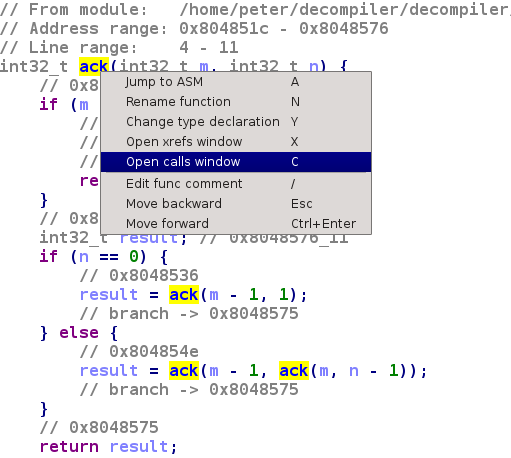
\includegraphics[width=7cm]{figures/context-actions-1-cut}
	\captionof{figure}{Context actions available for functions.}
	\label{fig:context-1}
\end{minipage}%
\begin{minipage}{.5\textwidth}
	\centering
	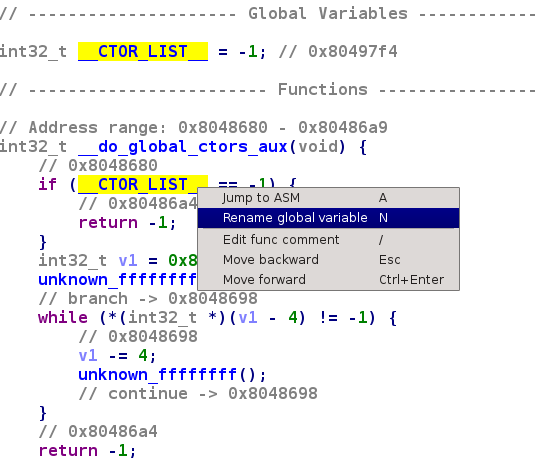
\includegraphics[width=7cm]{figures/context-actions-2-cut}
	\captionof{figure}{Context actions available for global variables.}
	\label{fig:context-2}
\end{minipage}
\end{figure}

%-----------------------------------------------------------------------------
%  List of All User Actions
%-----------------------------------------------------------------------------
\section{List of All User Actions}
\label{sec:all-interaction}
This section provides a complete catalog of available user actions for all possible contexts.

\subsection{Function-Declaration/Definition Context}
\label{sec:context-fnc-def}
Function actions are available on function declarations or definitions. They are listed in Table~\ref{table:function-context}.

\begin{table}[!ht]
\centering
\caption{Function context user actions.}
\label{table:function-context}
\begin{tabular}{llc}
\textbf{Action description} & \textbf{Hotkey} & \textbf{Triggers}\\
& & \textbf{re-decompilation}\\
\hline
Jump to IDA's ASM & \texttt{A} & \xmark \\
Rename function & \texttt{N} & \xmark \\
Change type declaration & \texttt{Y} & \cmark \\
Open xrefs window & \texttt{X} & \xmark \\
Open calls window & \texttt{C} & \xmark \\
\end{tabular}
\end{table}

\subsection{Function-Call Context}
Function-call actions are available on function calls. We can divide them into two categories:
\begin{itemize}
	\item Calls of user defined functions---actions are the same as in function-declaration/definition context (Section~\ref{sec:context-fnc-def}), except the ``Change type declaration'' action. Also, you can double-click on a call to decompile/display the called function.
	\item Calls of dynamically linked functions---the only available action is double-click, which takes you on the import stub in the IDA's disassembly view.
\end{itemize}

\subsection{Global-Variable Context}
Global-variable actions are available on global-variable definitions and uses. They are listed in Table~\ref{table:global-var-context}.

\begin{table}[!ht]
\centering
\caption{Global-variable context user actions.}
\label{table:global-var-context}
\begin{tabular}{llc}
\textbf{Action description} & \textbf{Hotkey} & \textbf{Triggers}\\
& & \textbf{re-decompilation}\\
\hline
Jump to IDA's ASM & \texttt{A} & \xmark \\
Rename global variable & \texttt{N} & \xmark
\end{tabular}
\end{table}

\subsection{Global Context}
Global context actions are available everywhere. They are listed in Table~\ref{table:global-context}.

\begin{table}[!ht]
\centering
\caption{Global context user actions.}
\label{table:global-context}
\begin{tabular}{llc}
\textbf{Action description} & \textbf{Hotkey} & \textbf{Triggers}\\
& & \textbf{re-decompilation}\\
\hline
Edit current function's comment & \texttt{;} & \xmark \\
Move backward (navigation) & \texttt{ESC} & \xmark \\
Move forward (navigation) & \texttt{CTRL+F} & \xmark
\end{tabular}
\end{table}

%-----------------------------------------------------------------------------
%  Support an Feedback
%-----------------------------------------------------------------------------
\section{Support and Feedback}
\label{sec:support}
RetDec plugin is still in an experimental beta version. If you have any feedback, suggestions, or bug reports, please open an issue in the GitHub project (preferred), or send them to us either through our website, or through email.
\begin{center}
{
\LARGE
\href{https://github.com/avast-tl/retdec-idaplugin}{https://github.com/avast-tl/retdec-idaplugin} \\[5 mm]
\href{https://retdec.com}{https://retdec.com} \\[5 mm]
\href{mailto:support@retdec.com}{support@retdec.com}
}
\end{center}

%-----------------------------------------------------------------------------
%  End of Document
%-----------------------------------------------------------------------------
\end{document}
